\documentclass[14pt]{extreport}
\usepackage{gost}
\usepackage{listings}
\usepackage{xcolor}
\usepackage{lscape}


\definecolor{codegreen}{rgb}{0,0.6,0}
\definecolor{codegray}{rgb}{0.5,0.5,0.5}
\definecolor{codepurple}{rgb}{0.58,0,0.82}
\definecolor{backcolour}{rgb}{0.95,0.95,0.92}

\lstdefinestyle{mystyle}{
    backgroundcolor=\color{backcolour},   
    commentstyle=\color{codegreen},
    keywordstyle=\color{magenta},
    numberstyle=\tiny\color{codegray},
    stringstyle=\color{codepurple},
    basicstyle=\ttfamily\footnotesize,
    breakatwhitespace=false,         
    breaklines=true,                 
    captionpos=b,                    
    keepspaces=true,                 
    numbers=left,                    
    numbersep=5pt,                  
    showspaces=false,                
    showstringspaces=false,
    showtabs=false,                  
    tabsize=2,
    texcl=true,
}

\lstset{style=mystyle}

\begin{document}
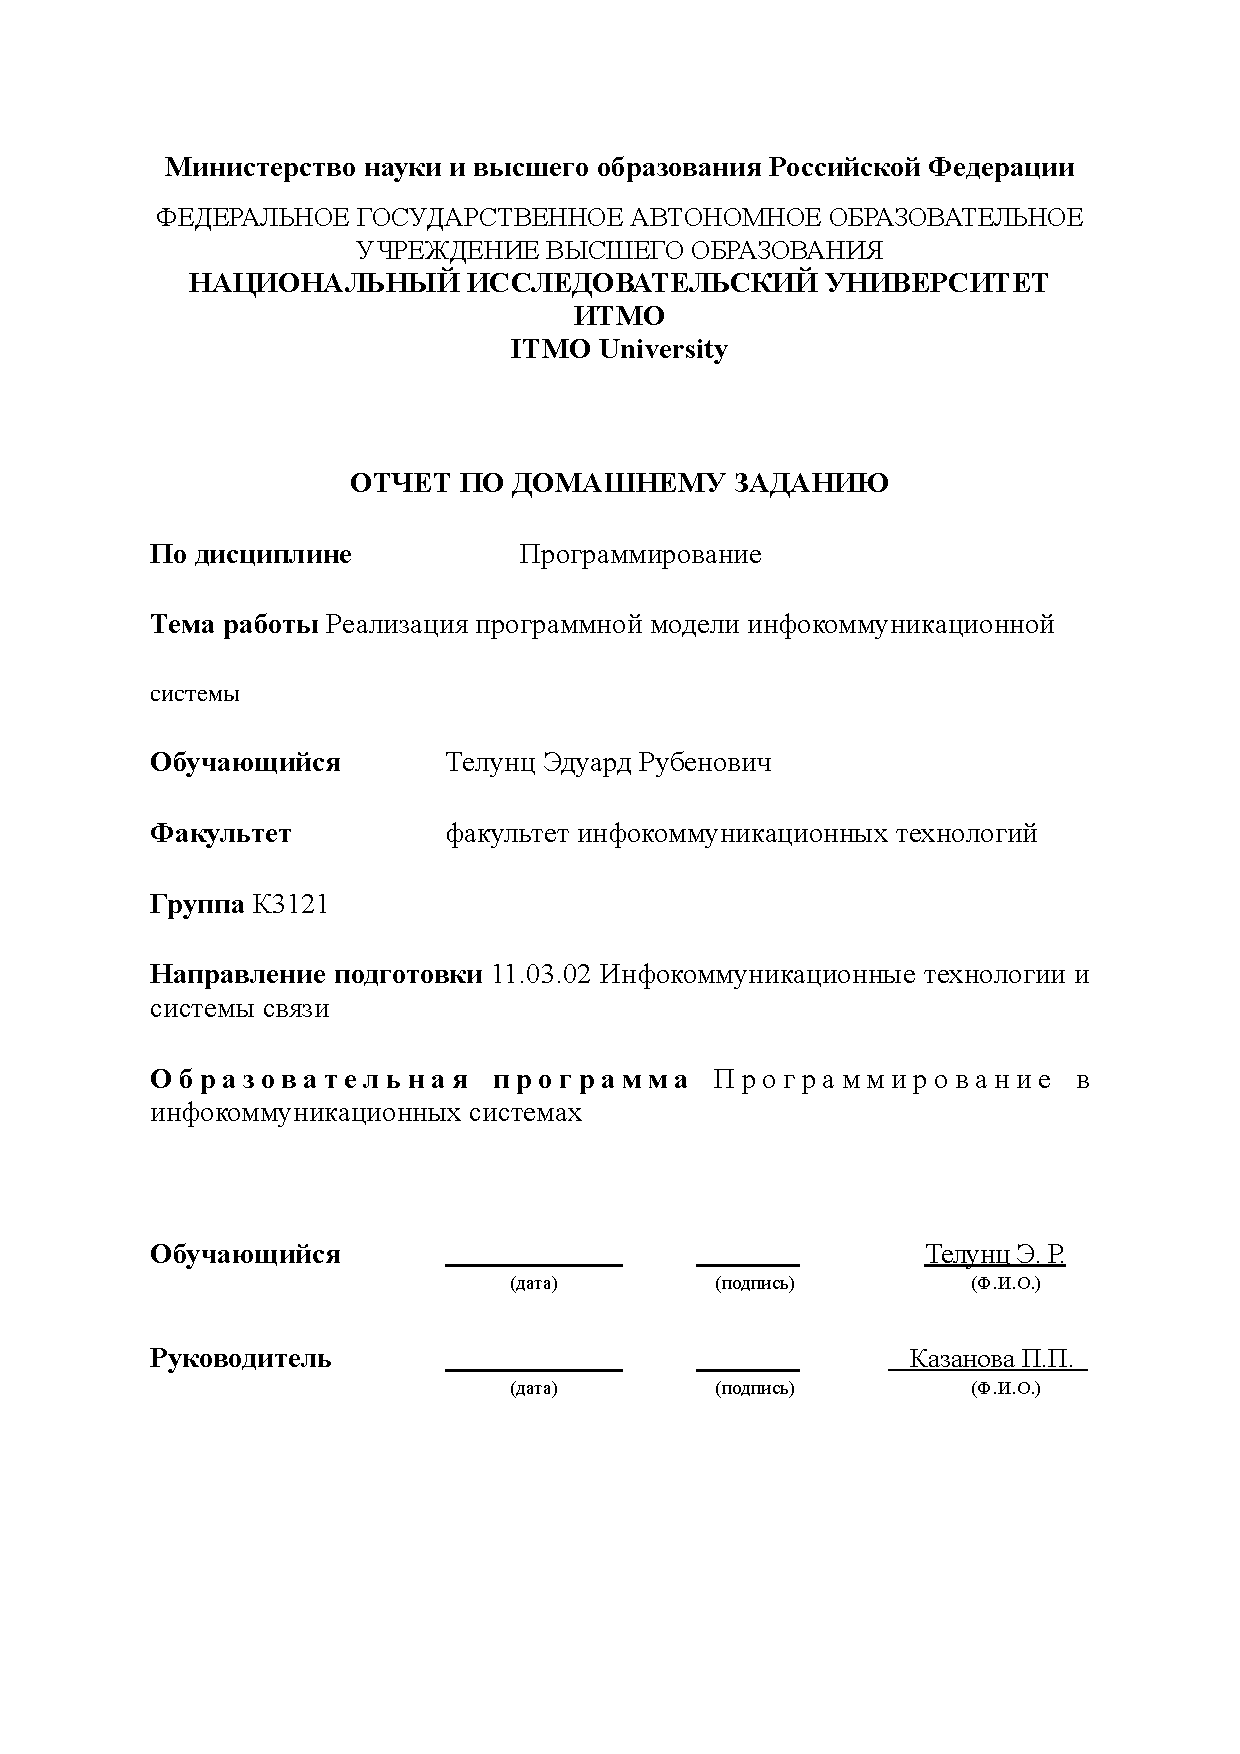
\includepdf[pages=-,pagecommand={}]{title_page.pdf}
\pagestyle{plain} % включаем нумерацию
\tableofcontents

\intro 
    Отчет по заданию "Учет грузового транспорта для логистической компании"

    Цель проекта: разработка программного обеспечения для учета грузового транспорта в Автотранспортном отделе логистической компании. Задача включала подбор доступного транспорта в зависимости от размера и веса груза с использованием ООП, БД и графического интерфейса.

    Реализованные функции:
    \begin{enumerate}
        \item Добавление/удаление грузового транспорта.
        \item Просмотр доступного транспорта.
        \item Просмотр транспорта по грузоподъемности.
        \item Просмотр свободного транспорта.
        \item Внесение заявки на перевоз груза по габаритам.
        \item Подбор и бронирование транспорта.
        \item Просмотр занятого транспорта.
        \item Реализация пользовательского интерфейса.
        \item Сохранение данных в базу данных.
    \end{enumerate}

\chapter{Ход работы}
    \section{Анализ предметной области и требований}
        Анализ предметной области и требований для задания "Учет грузового транспорта для логистической компании"

        Предметная область данного задания связана с учетом грузового транспорта в логистической компании. Главной целью программного обеспечения является облегчение и оптимизация процесса подбора и учета грузовых транспортных средств в зависимости от их грузоподъемности и доступности.

        Анализируя предметную область и требования к программному обеспечению, можно выделить следующие основные аспекты:

        \begin{enumerate}
            \item Учет грузового транспорта: Система должна позволять вести учет всех грузовых транспортных средств, которые находятся в распоряжении логистической компании. Для этого требуется функционал добавления и удаления транспорта, а также отображение общего списка доступных транспортных средств.
            \item Подбор транспорта по грузоподъемности: Одним из главных требований является возможность подбора подходящего грузового транспорта в зависимости от грузоподъемности. Это позволяет оптимизировать использование транспортных средств и избежать перегрузки или недоиспользования.
            \item Бронирование транспорта: Система должна предоставлять возможность бронирования выбранного транспортного средства для конкретной перевозки. Это позволяет удостовериться в его доступности и избежать конфликтов при назначении грузов на разные транспортные средства.
            \item Заявки на перевозку: Пользователи должны иметь возможность внести заявку на перевозку груза, указав его габариты и требования. Система должна уметь обрабатывать и анализировать эти заявки для более точного подбора транспорта и планирования перевозок.
            \item Интерфейс и БД: Важным требованием является реализация графического интерфейса, который обеспечит удобство использования системы и наглядность представления информации. Также требуется использование базы данных для хранения и управления информацией о грузовых транспортных средствах, заявках на перевозку и других связанных данных.
        \end{enumerate}

        Анализ предметной области и требований позволяет определить основные задачи, которые должны быть реализованы в разрабатываемом программном обеспечении, а также выбрать подходящие технологии и методы для их выполнения.

    \section{Выбор инструментов разработки}

        Язык программирования: Для реализации программного обеспечения был выбран язык программирования Python. Python является популярным языком с отличной поддержкой объектно-ориентированного программирования и обширной библиотекой сторонних модулей, что делает его удобным выбором для данного проекта.

        Графический интерфейс: Для реализации графического интерфейса был выбран модуль Tkinter, который является стандартной библиотекой Python. Tkinter обладает простым синтаксисом и хорошо подходит для создания базовых интерфейсов. Он также обеспечивает совместимость с различными платформами.

        База данных: В качестве системы управления базами данных (СУБД) был выбран PostgreSQL. PostgreSQL является мощной и надежной СУБД с открытым исходным кодом. Она поддерживает широкий спектр функциональных возможностей, включая сложные запросы и транзакции, что делает ее подходящим выбором для приложений учета и хранения данных.

        Работа с базой данных: Для работы с базой данных PostgreSQL был выбран SQLAlchemy, который является популярным ORM (объектно-реляционное отображение) для Python. SQLAlchemy предоставляет высокоуровневый интерфейс для взаимодействия с базой данных, а также упрощает выполнение запросов, создание таблиц и миграцию данных.

        Выбранные инструменты (Python, Tkinter, PostgreSQL и SQLAlchemy) обеспечивают удобство разработки, гибкость и мощные возможности для реализации требуемого функционала учета грузового транспорта в логистической компании.

    \section{Модели данных и взаимодействие с базой данных}
        Основой программы являются классы, описанные в представленном коде. Эти классы определяют модели данных для учета грузового транспорта и заявок на перевозку в логистической компании. Код использует ORM SQLAlchemy для работы с базой данных PostgreSQL, что обеспечивает удобный способ взаимодействия с данными и создания таблиц в базе данных. Реализация классов и их связей предоставляет основу для эффективного учета и управления грузовым транспортом, а также обработки заявок на перевозку.

        \begin{lstlisting}[language=Python]
Base = declarative_base()
engine = create_engine(f"postgresql+psycopg2://{DB_USER}:{DB_PASS}@{DB_HOST}:{DB_PORT}/{DB_NAME}")
        \end{lstlisting}
        \begin{center}
            Рисунок 1 - Определение SQLAlchemy
        \end{center}

        Данный код (Рисунок 1) устанавливает основу для определения моделей базы данных с использованием SQLAlchemy. Он создает базовый класс Base, от которого будут наследоваться все модели. Затем создается экземпляр engine, который представляет собой соединение с базой данных PostgreSQL. В строке подключения используются значения переменных DB USER, DB PASS, DB HOST, DB PORT и DB NAME, которые содержат информацию о пользователях, пароле, хосте, порте и названии базы данных соответственно. Этот engine будет использоваться для взаимодействия с базой данных при выполнении запросов и создании таблиц на основе определенных моделей.

        В представленном ниже коде определены классы, описывающие модели данных для учета грузового транспорта и заявок на перевозку. Используется ORM SQLAlchemy для работы с базой данных PostgreSQL.

        \begin{figure}[H]
            \centering
            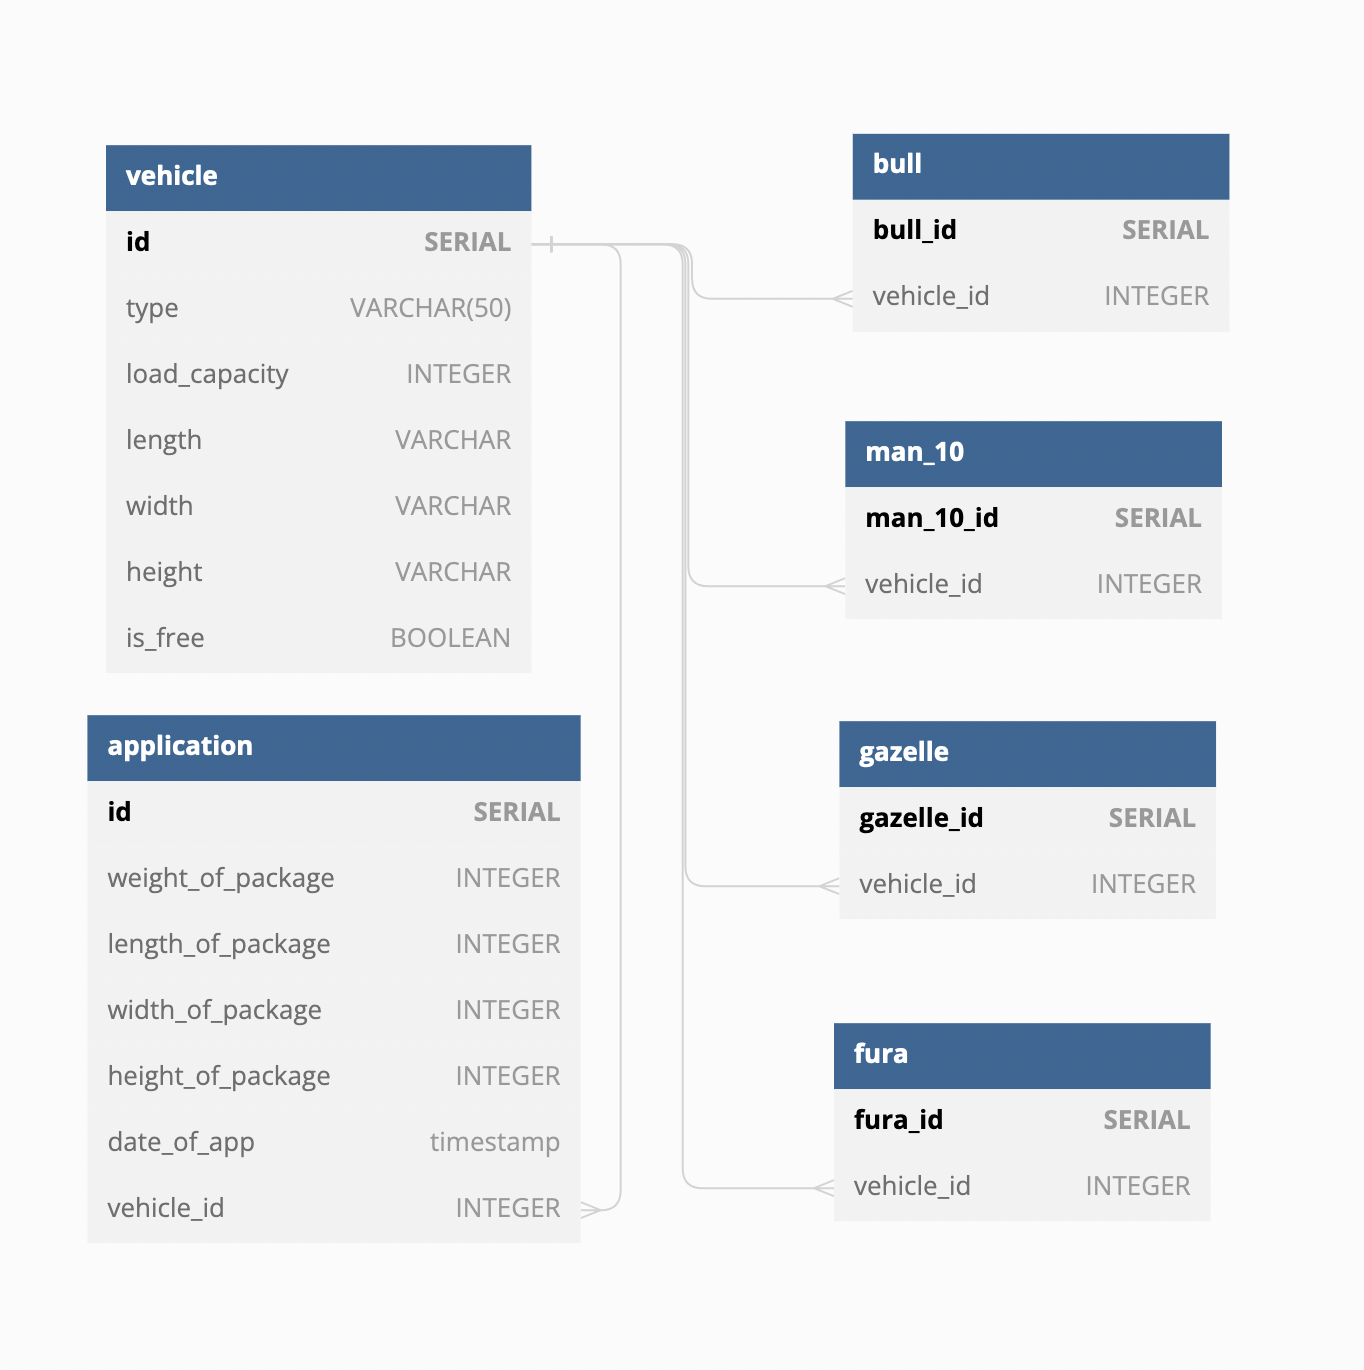
\includegraphics[scale=0.4]{db.png}
        \end{figure}
        \begin{center}
            Рисунок 2 - Схема базы данных
        \end{center}

    Таблица "vehicle" содержит информацию о транспортных средствах, таких как тип, грузоподъемность, длина, ширина, высота и статус доступности.

    Таблицы "gazelle", "bull", "man-10" и "fura" являются наследниками таблицы "vehicle" и содержат специфическую информацию для каждого типа транспортного средства.

    Таблица "application" хранит информацию о заявках, включая вес, размеры груза, дату подачи заявки и связь с соответствующим транспортным средством.

Связи между таблицами установлены с помощью внешних ключей. Например, каждая заявка в таблице "application" связана с конкретным транспортным средством из таблицы "vehicle".

        \subsection{Класс Vehicle}
        Класс "Vehicle" представляет общую модель для всех грузовых транспортных средств. Он содержит различные характеристики транспорта, такие как тип, грузоподъемность, размеры, а также флаг, указывающий на доступность транспорта. Он также имеет отношения с различными подклассами, такими как "Gazelle", "Bull", "MAN-10" и "Fura".

        \begin{lstlisting}[language=Python]
class Vehicle(Base):
    __tablename__ = 'vehicle'    
    id = Column(Integer, primary_key=True, nullable=False)
    type = Column(String(50))
    load_capacity = Column('load_capacity', Integer, nullable=False)
    length = Column('length', String, nullable=False)
    width = Column('width', String, nullable=False)
    height = Column('height', String, nullable=False)
    is_free = Column('is_free', Boolean, nullable=False, default=True)
    gazelle = relationship('Gazelle', backref='vehicle', passive_deletes=True)
    bull = relationship('Bull', backref='vehicle', passive_deletes=True)
    man_10 = relationship('MAN_10', backref='vehicle', passive_deletes=True)
    fura = relationship('Fura', backref='vehicle', passive_deletes=True)
    application = relationship('Application', backref='vehicle', passive_deletes=True)    
    __mapper_args__ = {
        'polymorphic_identity': 'vehicle',
        'polymorphic_on': type
    }
        \end{lstlisting}
    \begin{center}
        Рисунок 3 - Класс Vehicle 
    \end{center}
    \subsection{Подклассы}
    Каждый подкласс (например, "Gazelle", "Bull", "MAN-10", "Fura") (Рисунок 4) представляет конкретный тип грузового транспорта и содержит дополнительные свойства, специфичные для этого типа. Каждый подкласс имеет отношение "vehicle", указывающее на родительский объект "Vehicle".

    \begin{lstlisting}[language=Python]
class Gazelle(Vehicle):
    __tablename__ = 'gazelle'
    gazelle_id = Column(Integer, primary_key=True)
    vehicle_id = Column('vehicle_id', Integer, ForeignKey('vehicle.id', ondelete='CASCADE'))
class Bull(Vehicle):
    __tablename__ = 'bull'
    bull_id = Column(Integer, primary_key=True)
    vehicle_id = Column('vehicle_id', Integer, ForeignKey('vehicle.id', ondelete='CASCADE'))
class MAN_10(Vehicle):
    __tablename__ = 'man_10'
    man_10_id = Column(Integer, primary_key=True)
    vehicle_id = Column('vehicle_id', Integer, ForeignKey('vehicle.id', ondelete='CASCADE'))
class Fura(Vehicle):
    __tablename__ = 'fura'
    fura_id = Column(Integer, primary_key=True)
    vehicle_id = Column('vehicle_id', Integer, ForeignKey('vehicle.id', ondelete='CASCADE'))
                \end{lstlisting}
            \begin{center}
                Рисунок 4 - Подклассы 
            \end{center}
            \subsection{Класс Application}
            Класс "Application" (рисунок 5) представляет заявку на перевозку груза. Он содержит информацию о весе и габаритах груза, а также дате подачи заявки. Он также имеет отношение "vehicle", указывающее на выбранный транспорт для данной заявки.


    \begin{lstlisting}[language=Python]
class Application(Base):
    __tablename__ = 'application'
    id = Column(Integer, primary_key=True)
    weight_of_package = Column(Integer, nullable=False)
    length_of_package = Column(Integer, nullable=False)
    width_of_package = Column(Integer, nullable=False)
    height_of_package = Column(Integer, nullable=False)
    date_of_app = Column(DateTime, default=datetime.utcnow())
    vehicle_id = Column('vehicle_id', Integer, ForeignKey('vehicle.id', ondelete='CASCADE'))
                        \end{lstlisting}
                    \begin{center}
                        Рисунок 5 - Класс Application
                    \end{center}

    В представленном коде определены модели данных, которые соответствуют таблицам в базе данных. Для каждой модели определены атрибуты, которые представляют столбцы в таблице. Например, модель "Vehicle" имеет атрибуты, такие как "id", "type", "load capacity" и другие, которые отображаются на соответствующие столбцы в таблице "vehicle".

    Для работы с базой данных создается сессия, используя класс "Session". Сессия предоставляет методы для выполнения различных операций, таких как добавление, удаление, обновление и запрос данных из базы данных.

    \subsection{Диаграмма классов}

    Для наглядного представления структуры и взаимосвязей классов, используемых в программе учета грузового транспорта, была создана диаграмма классов (Рисунок 6). Диаграмма классов является графическим инструментом, который позволяет визуализировать классы, их атрибуты и методы, а также связи между классами.

    \begin{figure}[H]
        \centering
        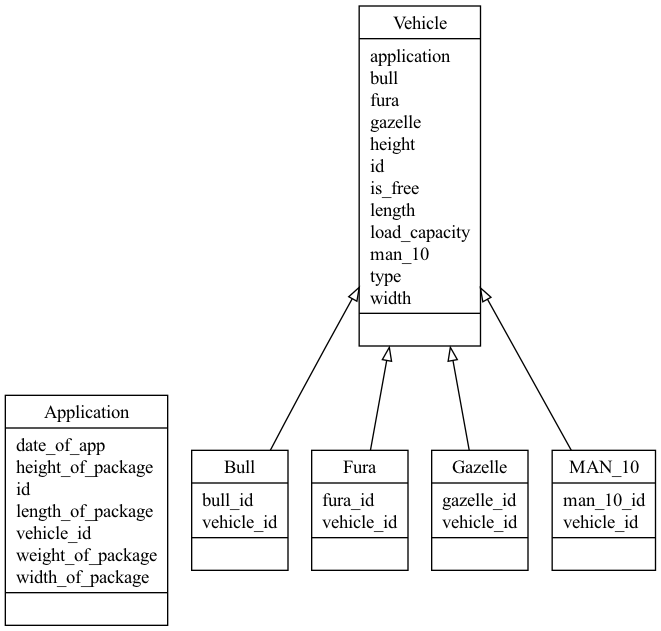
\includegraphics[scale=0.5]{classes_Vehicle.png}
    \end{figure}
    \begin{center}
        Рисунок 6 - Диаграмма классов 
    \end{center}

    В данной программе диаграмма (рисунок 6) классов представляет модели данных, которые используются для хранения информации о грузовом транспорте и заявках на перевозку. Она помогает понять структуру данных, их взаимосвязи и иерархию классов.

    \section{Разработка графического интерфейса}

    В данной программе реализован интерфейс (рисунок 7) для программы учета грузового транспорта. Он основан на библиотеке Tkinter и предоставляет возможности для добавления, удаления и просмотра данных о грузовых автомобилях.

Интерфейс состоит из нескольких элементов, которые размещены в окне программы. Пользователь может выбрать нужную функцию, нажав на кнопку "Возможности". После этого отображаются вкладки с различными функциональными блоками.
\begin{figure}[H]
    \centering
    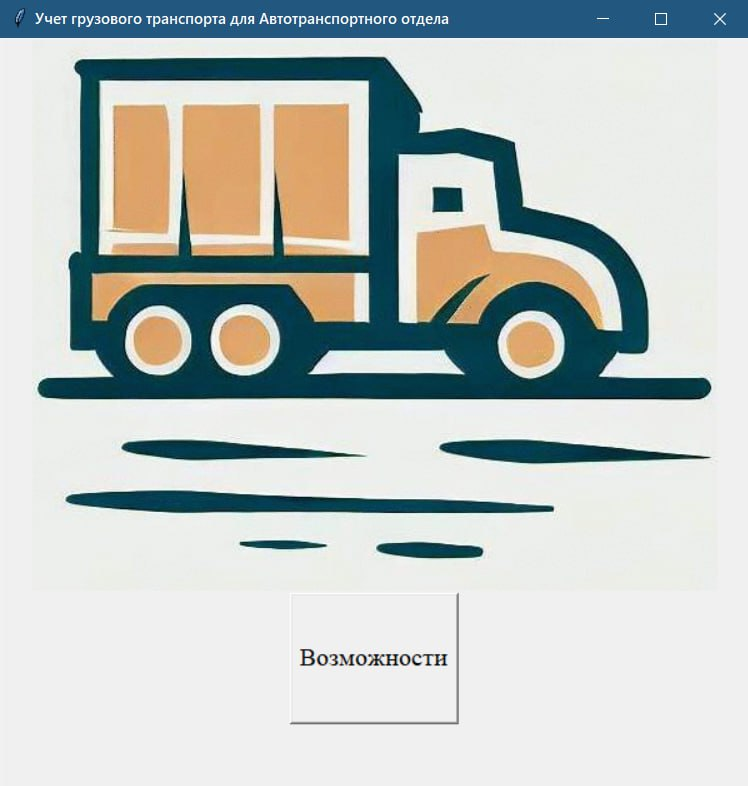
\includegraphics[scale=0.7]{1.jpg}
\end{figure}
\begin{center}
    Рисунок 7 - Стартовый экран
\end{center}

\subsection{Добавление и удаление}

В блоке "Добавление и удаление" (рисунок 8) пользователь может добавить новую запись о грузовом транспорте, выбрав тип грузовика (Газель, Бычок, MAN-10, Фура) и указав грузоподъемность, длину, ширину и высоту. После заполнения полей необходимо нажать кнопку "Добавить". Также есть возможность удалить записи, указав критерии поиска.

\begin{figure}[H]
    \centering
    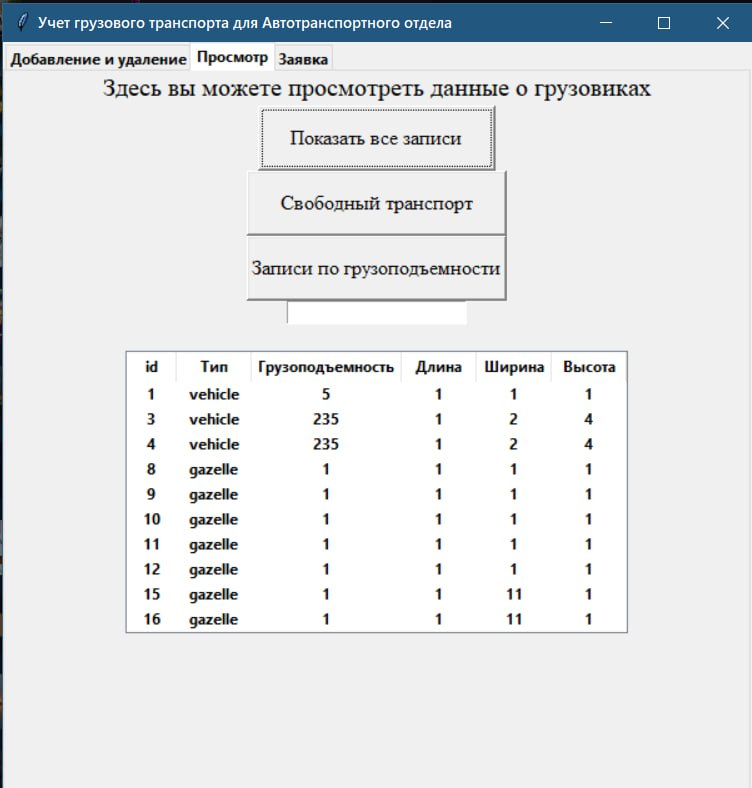
\includegraphics[scale=0.7]{2.jpg}
\end{figure}
\begin{center}
    Рисунок 8 - Добавление и удаление 
\end{center}

\subsection{Просмотр}

В блоке "Просмотр" (рисунок 9) пользователь может просмотреть все записи о грузовых автомобилях или отфильтровать их по грузоподъемности. Результат отображается в виде таблицы с колонками, представляющими различные атрибуты транспорта (ID, тип, грузоподъемность, длина, ширина, высота).

\begin{figure}[H]
    \centering
    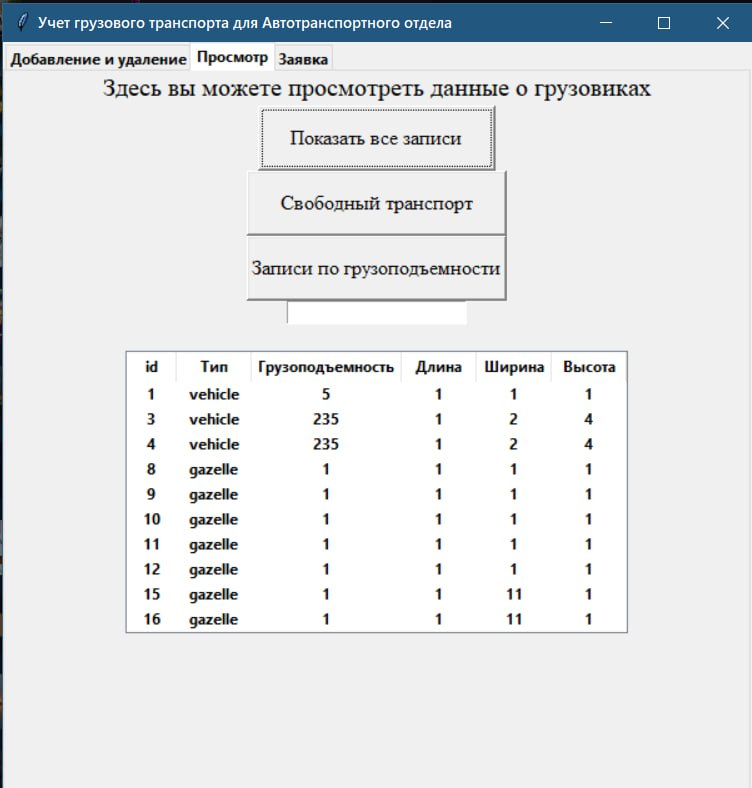
\includegraphics[scale=0.7]{3.jpg}
\end{figure}
\begin{center}
    Рисунок 9 - Просмотр
\end{center}

\subsection{Заявка}

В блоке "Заявка" (рисунок 10) пользователь может создать заявку на перевозку груза, указав параметры груза (вес, длину, ширину, высоту). Программа автоматически найдет подходящий свободный грузовик с достаточной грузоподъемностью и размерами для перевозки и добавит заявку в базу данных.

\begin{figure}[H]
    \centering
    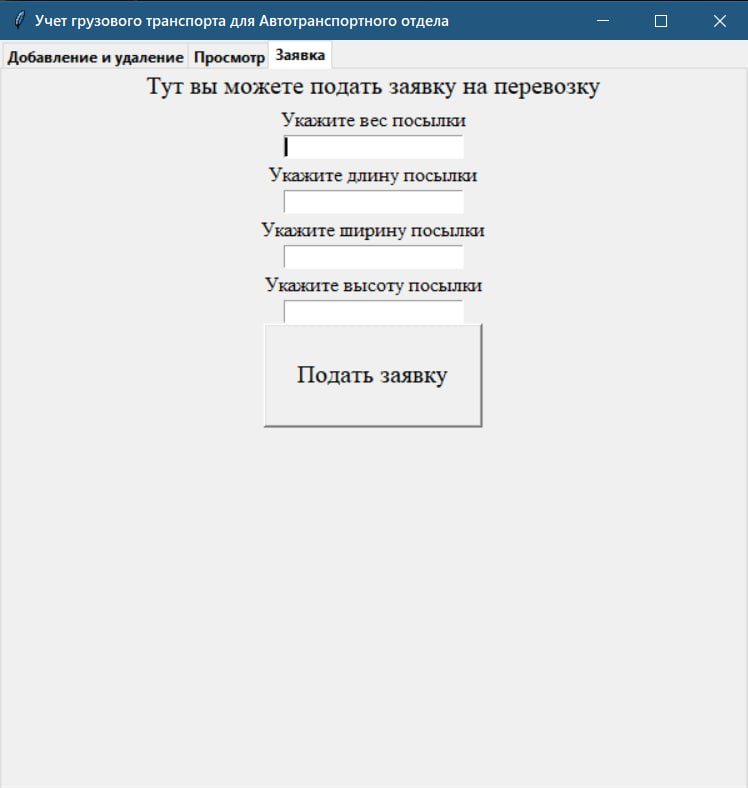
\includegraphics[scale=0.7]{4.jpg}
\end{figure}
\begin{center}
    Рисунок 10 - Заявка
\end{center}

Также в программе реализованы дополнительные функции, такие как отображение инструкции, валидация вводимых данных и обновление интерфейса в соответствии с выбранной функцией.

Этот код является основой для разработки интерфейса программы учета грузового транспорта и может быть доработан и расширен усмотрению.


\section{Разработка функционала приложения}
В процессе разработки приложения для учета грузового транспорта в автотранспортном отделе, определены следующие функции и их реализации:



1. Функция `check(s)`:
   - Выполняет проверку корректности введенных значений для длины, ширины и высоты транспорта. (Рисунок 11)
   \begin{lstlisting}[language=Python]
    def check(s):
        elements = s.split('-')
        if (len(elements) == 2) and (elements[0].isdigit()) and (elements[1].isdigit()) and (
                int(elements[0]) > int(elements[1])):
            return False
        else:
            return True
   \end{lstlisting}
   \begin{center}
    Рисунок 11 - Функция `check(s)`:
\end{center}
2. Функция `replacing(s)`:
   - Удаляет символ "\--" из строки. (Рисунок 12)
   \begin{lstlisting}[language=Python]
    def replacing(s):
        if (len(s) > 0) and (s[len(s) - 1] == '-'):
            s = s[:len(s) - 1]
        return s
   \end{lstlisting}
   \begin{center}
    Рисунок 12 - Функция `replacing(s)`:
\end{center}
3. Функция `adding()`:
   - Добавляет информацию о транспорте в базу данных. (Рисунок 13)
   \begin{lstlisting}[language=Python]
    def adding():
        type_of_transport = combox_type.get()
        load_capacity = entry_load_capacity.get()
        length = entry_length.get()
        width = entry_width.get()
        height = entry_height.get()

        if (len(type_of_transport) == 0) or (len(load_capacity) == 0) or (len(length) == 0) or \
                (len(width) == 0) or (len(height) == 0):
        elif (check(length)) and (check(width)) and (check(height)):
            length = replacing(length)
            width = replacing(width)
            height = replacing(height)
            new_vehicle = None
            if (type_of_transport == "gazelle"):
                new_vehicle = Gazelle(load_capacity=load_capacity, length=length, width=width, height=height)
            elif (type_of_transport == "bull"):
                new_vehicle = Bull(load_capacity=load_capacity, length=length, width=width, height=height)
            elif (type_of_transport == "MAN-10"):
                new_vehicle = MAN_10(load_capacity=load_capacity, length=length, width=width, height=height)
            elif (type_of_transport == "fura"):
                new_vehicle = Fura(load_capacity=load_capacity, length=length, width=width, height=height)

            session.add(new_vehicle)
            session.commit()
   \end{lstlisting}
   \begin{center}
    Рисунок 13 - Функция `adding()`:
\end{center}
4. Функция `deleting()`:
   - Удаляет информацию о транспорте из базы данных. (Рисунок 14)
   \begin{lstlisting}[language=Python]
    def deleting():
        type_of_transport = combox_type.get()
        load_capacity = entry_load_capacity.get()
        length = entry_length.get()
        width = entry_width.get()
        height = entry_height.get()

        if (len(type_of_transport) == 0) and (len(load_capacity) == 0) and (len(length) == 0) and \
                (len(width) == 0) and (len(height) == 0):

        elif (check(length)) and (check(width)) and (check(height)):
            length = replacing(length)
            width = replacing(width)
            height = replacing(height)

            request = session.query(Vehicle)
            if (type_of_transport != ""):
                request = request.filter(type_of_transport == Vehicle.type)
            if (load_capacity != ""):
                request = request.filter(load_capacity == Vehicle.load_capacity)
            if (length != ""):
                request = request.filter(length == Vehicle.length)
            if (width != ""):
                request = request.filter(width == Vehicle.width)
            if (height != ""):
                request = request.filter(height == Vehicle.height)

        request.delete()
        session.commit()
   \end{lstlisting}
   \begin{center}
    Рисунок 14 - Функция `deleting()`:
\end{center}
5. Функция `show all()`:
   - Отображает все записи о транспорте из базы данных. (Рисунок 15)
   \begin{lstlisting}[language=Python]
    def show_all():
        tree.pack()
        request = session.query(Vehicle)

        tree.delete(*tree.get_children())

        for i in request:
            tree.insert(parent='', index='end', text='', values=(str(i.id), i.type, str(i.load_capacity), i.length, i.width, i.height))
   \end{lstlisting}
   \begin{center}
    Рисунок 15 - Функция `show all()`:
\end{center}
6. Функция `show load capacity()`:
   - Отображает записи о транспорте с заданной грузоподъемностью. (Рисунок 16)
   \begin{lstlisting}[language=Python]
def show_load_capacity():
    load_capacity_interval = entry_showing_load_capacity.get().split('-')
    if (len(load_capacity_interval) == 2) and (load_capacity_interval[1] == ''):
        load_capacity_interval.remove('')
    elif (len(load_capacity_interval) == 1):
        tree.pack()

        load_capacity = int(load_capacity_interval[0])
        request = session.query(Vehicle).filter(load_capacity == Vehicle.load_capacity)
        tree.delete(*tree.get_children())

        for i in request:
            tree.insert(parent='', index='end', text='', values=(str(i.id), i.type, str(i.load_capacity), i.length, i.width, i.height))

    elif (len(load_capacity_interval) == 2):
        tree.pack()

        start = int(load_capacity_interval[0])
        end = int(load_capacity_interval[1])

        request = session.query(Vehicle).filter(start <= Vehicle.load_capacity).filter(Vehicle.load_capacity <= end)
        tree.delete(*tree.get_children())

        for i in request:
            tree.insert(parent='', index='end', text='', values=(str(i.id), i.type, str(i.load_capacity), i.length, i.width, i.height))

   \end{lstlisting}
   \begin{center}
    Рисунок 16 - Функция `show load capacity()`:
\end{center}
7. Функция `show free()`:
   - Отображает записи о свободном транспорте. (Рисунок 17)
   \begin{lstlisting}[language=Python]
    def show_free():
        tree.pack()
        request = session.query(Vehicle).filter(Vehicle.is_free == True)
        tree.delete(*tree.get_children())
        for i in request:
            tree.insert(parent='', index='end', text='', values=(str(i.id), i.type, str(i.load_capacity), i.length, i.width, i.height))
   \end{lstlisting}
   \begin{center}
    Рисунок 17 - Функция `show free()`:
\end{center}
8. Функция `application()`:
    - Добавляет заявку в базу данных и находит подходящий транспорт. (Рисунок 18)
    \begin{lstlisting}[language=Python]
    def application():
        weight = entry_weight_app.get()
        length = entry_length_app.get()
        width = entry_width_app.get()
        height = entry_height_app.get()
    
        if (weight == '') or (length == '') or (width == '') or (height == ''):
            lbl_app_result.config(text="error")
        else:
            weight, length, width, height = int(weight), int(length), int(width), int(height)
    
            request = session.query(Vehicle).filter(Vehicle.load_capacity >= weight).filter(Vehicle.is_free == True)
            min_volume = math.inf
            need_id = -1
    
            for i in request:
                length_r = int(i.length.split('-')[-1])
                width_r = int(i.width.split('-')[-1])
                height_r = int(i.height.split('-')[-1])
    
                if (length_r >= length) and (width_r >= width) and (height_r >= height) and (length_r*width_r*height_r <= min_volume):
                    min_volume = length_r*width_r*height_r
                    need_id = i.id
    
            if (need_id == -1):
                lbl_app_result.config(text="error")
            else:
                vehicle = session.get(Vehicle, need_id)
                vehicle.is_free = False
                
                app = Application(weight_of_package=weight, length_of_package=length, width_of_package=width, height_of_package=height, vehicle_id=need_id)
                session.add(app)
                session.commit()
    \end{lstlisting}
    \begin{center}
        Рисунок 18 - Функция `Application()`:
    \end{center}
9. Функция `validate load capacity(P)`:
    - Выполняет валидацию введенных значений для грузоподъемности. (Рисунок 19)
    \begin{lstlisting}[language=Python]
        def validate_load_capacity(P):
            if P.isdigit() or P == "":
                return True
            else:
                return False
    \end{lstlisting}
    \begin{center}
        Рисунок 19 - Функция `validate load capacity()`:
    \end{center}
10. Функция `validate parameters(P)`:
    - Выполняет валидацию введенных значений для параметров транспорта. (Рисунок 20)
    \begin{lstlisting}[language=Python]
        def validate_parameters(P):
            result = re.fullmatch(r"\d+-?\d*", P)
            if (result) or (P == ""):
                return True
            else:
                return False
    \end{lstlisting}
    \begin{center}
        Рисунок 20 - Функция `validate parameters(s)`:
    \end{center}
Каждая из этих функций имеет свою задачу и вместе они обеспечивают функциональность и удобство использования приложения для учета грузового транспорта.

\conclusions

В ходе выполнения задания было разработано программное обеспечение для учета грузового транспорта в Автотранспортном отделе логистической компании. Приложение было реализовано с использованием концепции объектно-ориентированного программирования (ООП), базы данных (БД) и графического интерфейса.

В результате работы были успешно выполнены все поставленные требования:
\begin{itemize}
    \item Реализована функциональность добавления и удаления грузового транспорта.
    \item Реализован просмотр всего доступного транспорта.
    \item Реализован просмотр грузового транспорта по грузоподъемности.
    \item Реализован просмотр свободного грузового транспорта.
    \item Реализована возможность внесения заявки на перевоз груза с указанием габаритов.
    \item Реализован алгоритм подбора и бронирования подходящего транспорта.
    \item Реализован просмотр занятого грузового транспорта.
    \item Разработан пользовательский интерфейс, соответствующий требованиям и обеспечивающий удобство использования.
    \item Реализована возможность сохранения данных в базу данных.
\end{itemize}

В целом, выполнение задания позволило создать функциональное и эффективное программное обеспечение, которое позволит автотранспортному отделу логистической компании управлять информацией о грузовом транспорте и заявках на перевозку.

\end{document}